%% Informe Entrega 2 - Proyecto B (glaucoma) - Imagenes Medicas 34740
%% Basado en la plantilla Springer Nature (sn-jnl), version 3.1 dic. 2024
%% Compilar en Overleaf con pdfLaTeX + BibTeX. Archivos necesarios:
%%   main.tex, referencias.bib (y figuras/ cuando existan).
%% Todo lo marcado con \pendiente{...} depende de la ejecucion del codigo
%% o de un dato que el equipo debe confirmar.

\documentclass[pdflatex,sn-mathphys-num]{sn-jnl}% Math and Physical Sciences Numbered Reference Style

\usepackage{graphicx}%
\usepackage{multirow}%
\usepackage{amsmath,amssymb,amsfonts}%
\usepackage{amsthm}%
\usepackage{mathrsfs}%
\usepackage[title]{appendix}%
\usepackage{xcolor}%
\usepackage{textcomp}%
\usepackage{manyfoot}%
\usepackage{booktabs}%
\usepackage{algorithm}%
\usepackage{algorithmicx}%
\usepackage{algpseudocode}%
\usepackage{listings}%
\usepackage{array}%
\usepackage{tabularx}%

%% Marcador para contenido que depende del codigo o de un dato por confirmar
\newcommand{\pendiente}[1]{\textcolor{red}{\textbf{[PENDIENTE: #1]}}}
%% Celda pendiente corta para tablas
\newcommand{\pend}{\textcolor{red}{\textbf{--}}}

\newcolumntype{L}[1]{>{\raggedright\arraybackslash}p{#1}}

\theoremstyle{thmstyleone}%
\newtheorem{theorem}{Theorem}%
\theoremstyle{thmstyletwo}%
\newtheorem{remark}{Remark}%
\theoremstyle{thmstylethree}%
\newtheorem{definition}{Definition}%

\raggedbottom
\setlength{\emergencystretch}{3em}% evita desbordes con nombres de archivo largos

\begin{document}

%% Nombres en espanol (sin babel, para no depender de la configuracion del compilador)
\renewcommand{\tablename}{Tabla}
\renewcommand{\figurename}{Figura}
\renewcommand{\refname}{Referencias}
\renewcommand{\appendixname}{Anexo}
\renewcommand{\contentsname}{Contenido}

%%==================================================================%%
%% PORTADA (no cuenta dentro de las 6-8 paginas de contenido)       %%
%%==================================================================%%
\begin{titlepage}
\centering
{\large\textbf{PONTIFICIA UNIVERSIDAD JAVERIANA}\par}
\vspace{0.3cm}
{Facultad de Ingeniería -- Programa de Bioingeniería\par}
\vspace{2.5cm}
{\Large\textbf{PROYECTO DE IMÁGENES MÉDICAS}\par}
\vspace{0.4cm}
{\Large\textbf{ENTREGA 2}\par}
\vspace{0.4cm}
{\large Del método elegido al primer resultado verificable\par}
\vspace{1.2cm}
{\large\textit{Proyecto B: Identificación de glaucoma en imágenes de fondo de ojo}\par}
\vspace{0.6cm}
{\large\textbf{Equipo} \pendiente{número de equipo}\par}
\vspace{2cm}
\begin{tabular}{rl}
\textbf{Asignatura:} & Imágenes Médicas -- 34740\\
\textbf{Profesor:}   & Xavier Díaz\\[0.4cm]
\textbf{Integrantes:} & Giuseppe Kanyike Buwule\\
                      & Daniel Duque\\
                      & Juan David Daza\\
\end{tabular}
\vfill
{Bogotá D.\,C., octubre de 2026\par}
\end{titlepage}

%%==================================================================%%
%% ENCABEZADO DEL ARTICULO (plantilla sn-jnl)                        %%
%%==================================================================%%
\title[Entrega 2 -- Proyecto B -- Glaucoma]{Clasificación de glaucoma en imágenes de fondo de ojo de ORIGA-light: datos, partición y primera línea base}

\author{\fnm{Giuseppe} \sur{Kanyike Buwule}}
\author{\fnm{Daniel} \sur{Duque}}
\author{\fnm{Juan David} \sur{Daza}}

\affil{\orgdiv{Facultad de Ingeniería, Programa de Bioingeniería}, \orgname{Pontificia Universidad Javeriana}, \orgaddress{\city{Bogotá D.\,C.}, \country{Colombia}}}

\abstract{Este informe documenta la segunda entrega del Proyecto B (equipo \pendiente{número}): el inventario real de la copia de ORIGA-light que usamos, la partición en entrenamiento, validación y prueba con su comprobación de solapamiento, la elección justificada de una línea base y su primera ejecución sobre el subconjunto de validación. La línea base describe cada imagen con ocho medidas de color y brillo de la región del disco óptico, entre ellas la palidez del centro frente al borde, y las clasifica con una regresión logística balanceada. En validación obtuvo un AUC de 0,667 (IC 95\,\%: 0,54--0,78), con sensibilidad de 0,70 y especificidad de 0,63. La comprobación de la partición encontró nueve pares de tomas del mismo ojo, cinco de ellos repartidos entre particiones; las cuatro imágenes de prueba afectadas se excluirán de la evaluación final. El conjunto de prueba se mantiene reservado. Los resultados se presentan como preliminares y no constituyen evidencia de eficacia clínica.}

\keywords{glaucoma, fondo de ojo, ORIGA-light, clasificación binaria, características de color, regresión logística}

\maketitle

%%==================================================================%%
\section{Datos utilizados}\label{sec:datos}
%%==================================================================%%

Trabajamos con ORIGA-light, el conjunto de fondo de ojo publicado por el Singapore Eye Research Institute (SERI) \cite{zhang2010origa}. Como la fuente oficial solo entrega los datos bajo solicitud y esa solicitud no fue respondida a tiempo, usamos una copia pública en Kaggle, tal como se explicó en la Entrega 1. Esta vez revisamos la copia completa con un script de inventario (\texttt{01\_inventario.py}, incluido en el ZIP de evidencias), que abre cada imagen, la cruza con los archivos CSV de etiquetas y calcula un hash MD5 por archivo. La Tabla~\ref{tab:datos} resume lo encontrado.

\begin{table}[h]
\caption{Resumen de la copia de datos utilizada}\label{tab:datos}
\begin{tabularx}{\textwidth}{@{}L{3.6cm}X@{}}
\toprule
Aspecto & Detalle \\
\midrule
Nombre y versión & \textit{ORIGA Retinal Fundus Image Dataset}, copia publicada en Kaggle por el usuario \texttt{ferencjuhsz}. La página no declara número de versión; se usa la versión disponible a la fecha de acceso. \\
Fuente original & ORIGA-light, SERI, descrito por Zhang et al.\ (2010) \cite{zhang2010origa}. Acceso oficial bajo solicitud. \\
Enlace & \url{https://www.kaggle.com/datasets/ferencjuhsz/origa-retinal-fundus-image-dataset} \cite{kaggleoriga} \\
Fecha de acceso & \pendiente{fecha de descarga} \\
Archivos & 650 imágenes JPG (454 en \texttt{ORIGA/train}, 196 en \texttt{ORIGA/test}) y 2 archivos CSV (\texttt{ORIGA\_train.csv}, \texttt{ORIGA\_test.csv}). \\
Casos y pacientes & 650 imágenes, cada una con un código numérico único entre 001 y 650. La copia no trae identificador de paciente ni de ojo, así que no es posible contar pacientes. \\
Etiquetas & Columna \texttt{glaucoma} con valores 0 (sano) y 1 (glaucoma): 168 positivas y 482 negativas. \\
Máscaras & No incluidas en esta copia. Los CSV solo tienen las columnas \texttt{ImageName} y \texttt{glaucoma}. \\
Características & Todas las imágenes son RGB y cuadradas, con 158 tamaños distintos entre 255$\times$255 y 493$\times$493 píxeles. Por inspección visual de una muestra, son recortes centrados en el disco óptico y no retinografías completas. \\
Faltantes, ilegibles, sin referencia, repetidos & 0 imágenes listadas en los CSV sin archivo; 0 archivos sin etiqueta; 0 archivos ilegibles; 0 nombres repetidos; 0 archivos con contenido idéntico (MD5). Sí hay repeticiones no exactas: 9 pares de imágenes son dos tomas del mismo ojo (Sección~\ref{sec:particion}). No se excluyó ninguna imagen del entrenamiento ni de la validación. \\
Condiciones de uso & La copia de Kaggle declara licencia MIT \cite{mitlicense}. La fuente original no publica términos de redistribución. \\
\botrule
\end{tabularx}
\end{table}

Respecto a la Entrega 1 hay una corrección: el rango de resolución que reportamos entonces (275$\times$275 a 443$\times$443) era una estimación hecha con unas pocas imágenes. El inventario completo da 255$\times$255 a 493$\times$493. También confirmamos que la copia no contiene las retinografías originales de alta resolución, sino recortes alrededor del disco óptico, lo cual influye en el preprocesamiento (Sección~\ref{sec:metodo}).

Los conteos por partición original de la copia coinciden con lo reportado en la Entrega 1: el subconjunto \texttt{train} tiene 454 imágenes (117 glaucoma, 337 sanas) y \texttt{test} tiene 196 (51 glaucoma, 145 sanas). El total de 168 casos de glaucoma coincide con la cifra de la publicación original, lo que respalda que la copia corresponde a ORIGA-light completo.

\paragraph{Permiso para compartir ejemplos.} Aunque la copia se distribuye con licencia MIT, no pudimos confirmar que el SERI autorice la redistribución. Por prudencia, el ZIP de evidencias \textbf{no incluye el conjunto de datos}: solo contiene el código, las tablas (que referencian las imágenes por su código, por ejemplo \texttt{train/093}) y las figuras con los tres casos ilustrativos y los pares de imágenes repetidas. Para reproducir el trabajo, el conjunto se descarga del enlace de la Tabla~\ref{tab:datos}.

%%==================================================================%%
\section{Separación de los datos}\label{sec:particion}
%%==================================================================%%

ORIGA-light no tiene una partición oficial única: distintos trabajos dividen las 650 imágenes de forma diferente. Decidimos respetar la división que trae la copia y construir la validación a partir del entrenamiento:

\begin{itemize}
\item \textbf{Prueba:} las 196 imágenes de \texttt{ORIGA/test}. No se han usado en ningún paso de este informe y quedan reservadas para la evaluación final.
\item \textbf{Validación:} 20\,\% de \texttt{ORIGA/train}, elegido con muestreo estratificado por etiqueta (función \texttt{train\_test\_split} de scikit-learn \cite{pedregosa2011scikit}, \texttt{test\_size=0.2}, \texttt{random\_state=42}), para conservar la proporción de glaucoma.
\item \textbf{Entrenamiento:} el 80\,\% restante de \texttt{ORIGA/train}. Es el único subconjunto con el que se ajusta el método.
\end{itemize}

La asignación queda guardada en \texttt{particion.csv}, con una fila por imagen (código, partición y etiqueta). La Tabla~\ref{tab:particion} muestra los conteos.

\begin{table}[h]
\caption{Conteos por partición. Como la copia no identifica pacientes, la unidad contada es la imagen}\label{tab:particion}
\begin{tabular*}{\textwidth}{@{\extracolsep\fill}lcccc}
\toprule
Partición & Imágenes & Glaucoma (1) & Sano (0) & \% glaucoma \\
\midrule
Entrenamiento & 363 & 94 & 269 & 25,9 \\
Validación    & 91  & 23 & 68  & 25,3 \\
Prueba (reservada) & 196 & 51 & 145 & 26,0 \\
\midrule
Total & 650 & 168 & 482 & 25,8 \\
\botrule
\end{tabular*}
\footnotetext{Los conteos de entrenamiento y validación corresponden a la división estratificada descrita en el texto y coinciden con la salida de \texttt{02\_particion.py}. De las 196 imágenes de prueba, 4 se excluirán de la evaluación final por tener un gemelo en entrenamiento (ver más abajo); la prueba efectiva será de 192 (49 glaucoma, 143 sanas).}
\end{table}

\subsection*{Comprobación de que un mismo caso no aparece en dos partes}

La guía pide mantener juntos ambos ojos y las visitas de una persona. En esta copia no podemos hacerlo directamente, porque no hay identificador de paciente ni indicación de ojo derecho o izquierdo, y no queremos inventar uno. En la Entrega 1 asumimos, con base en la descripción de la fuente, que cada imagen corresponde a una persona distinta. Las comprobaciones de esta entrega muestran que esa suposición \textbf{no se cumple del todo}.

Con el script \texttt{03\_verificar\_particion.py} comprobamos:

\begin{enumerate}
\item \textbf{Códigos de imagen:} la intersección de nombres entre entrenamiento, validación y prueba es vacía.
\item \textbf{Archivos idénticos:} no hay dos archivos con el mismo hash MD5 en todo el conjunto, ni dentro de una partición ni entre particiones.
\item \textbf{Casi duplicados:} se calcula un hash perceptual (pHash de 64 bits) de cada imagen y se listan los pares cuya distancia de Hamming sea menor o igual a 8. Entre particiones distintas se compararon 122\,017 pares (mediana de la distancia: 28) y 4 quedaron bajo el umbral; dentro de una misma partición quedaron otros 5, que no son fuga pero sí repeticiones. Al revisarlos a ojo, observamos que las repeticiones aparecían con números de imagen vecinos, así que añadimos una segunda búsqueda: los 649 pares de códigos consecutivos ($n$, $n+1$) con distancia menor o igual a 12. Encontramos 8 pares, uno de ellos (\texttt{train/026} y \texttt{train/027}) por encima del primer umbral.
\end{enumerate}

Revisamos visualmente todos los pares marcados. \textbf{Nueve pares son dos tomas del mismo ojo}: muestran el mismo trazado de vasos, con distinta exposición o un recorte algo desplazado. Cuatro quedan dentro de entrenamiento y cinco cruzan particiones (Figura~\ref{fig:pares}): uno entre entrenamiento y validación (\texttt{train/026}--\texttt{train/027}) y cuatro entre entrenamiento y prueba (\texttt{test/158}, \texttt{test/170}, \texttt{test/181} y \texttt{test/313}). Otros dos pares marcados resultaron ser ojos distintos y uno (\texttt{train/147}--\texttt{test/175}) quedó como dudoso. En uno de los pares internos de entrenamiento (\texttt{train/050}--\texttt{train/052}) las dos tomas tienen \textbf{etiquetas distintas} (glaucoma y sano). Con esta copia no podemos saber si es un error de etiqueta o si son tomas de momentos distintos con diagnósticos distintos, pero en cualquier caso muestra que las etiquetas no son del todo consistentes. La conclusión de la revisión queda registrada en \texttt{config.yaml} y en \texttt{revision\_pares.csv}.

\begin{figure}[h]
\centering
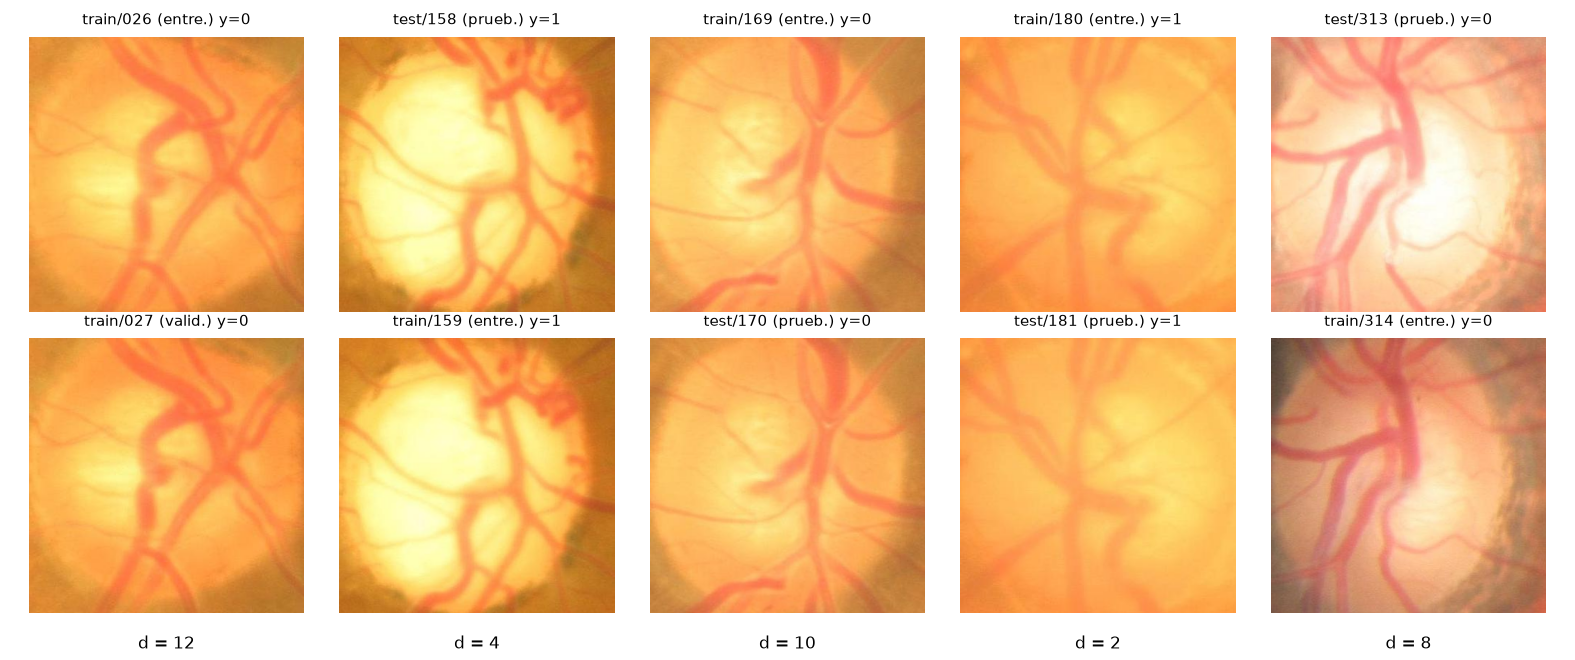
\includegraphics[width=\textwidth]{figuras/pares_mismo_ojo.png}
\caption{Los cinco pares del mismo ojo que cruzan particiones. Cada columna es un par (arriba y abajo), con su partición, su etiqueta ($y$) y la distancia pHash ($d$)}\label{fig:pares}
\end{figure}

\textbf{Decisión.} Mantenemos la partición (363/91/196) para no cambiar el diseño ya planteado, y tratamos la fuga así: (i) las 4 imágenes de prueba con un gemelo en entrenamiento se \textbf{excluirán de la evaluación final}, que se hará sobre 192 imágenes (lista en \texttt{prueba\_excluidos.csv}); (ii) el caso de validación \texttt{train/027} se mantiene, pero reportamos su efecto en la Sección~\ref{sec:piloto}. El pHash no detecta los dos ojos de una misma persona, que pueden verse distintos. Para resolverlo de fondo, mantenemos la solicitud de acceso al SERI, cuya versión podría traer el identificador de paciente y el ojo. Si llega antes de la entrega final, repetiremos la partición agrupando por paciente.

\subsection*{Cómo evitamos la fuga de datos}

Todo lo que se aprende de los datos se estima solo con el subconjunto de entrenamiento: la media y la desviación usadas para estandarizar las características y los coeficientes de la regresión logística. Los demás parámetros (tamaño de imagen, radios de las regiones, $C=1$ y umbral de 0,5) se fijaron de antemano y no se ajustaron mirando la validación. La validación se usa una sola vez, para el resultado de la Sección~\ref{sec:piloto}, y la prueba no se ha tocado: para buscar repeticiones solo se usaron los archivos, no las predicciones del modelo.

%%==================================================================%%
\section{Método elegido}\label{sec:metodo}
%%==================================================================%%

\subsection{Trabajos técnicos de referencia}

La Tabla~\ref{tab:estado} resume tres trabajos que abordan la detección de glaucoma en fondo de ojo y que sirven de punto de comparación para nuestra elección.

\begin{table}[h]
\caption{Comparación de trabajos técnicos relacionados}\label{tab:estado}
\begin{tabularx}{\textwidth}{@{}L{2.6cm}XXX@{}}
\toprule
Autor y año & Datos y tarea & Método y métrica & Limitación para nuestro proyecto \\
\midrule
\pendiente{1} & \pend & \pend & \pend \\
\pendiente{2} & \pend & \pend & \pend \\
\pendiente{3} & \pend & \pend & \pend \\
\botrule
\end{tabularx}
\end{table}

\pendiente{Párrafo breve que relacione los tres trabajos con nuestra decisión: qué tomamos de cada uno y por qué no lo replicamos tal cual.}

\subsection{Por qué esta línea base}

Para detectar glaucoma en fondo de ojo, la literatura sigue sobre todo dos caminos. El primero segmenta el disco y la copa ópticos y calcula la relación copa/disco (CDR). El segundo clasifica la imagen con una red convolucional. Para esta primera prueba no usamos ninguno de los dos y empezamos por algo más simple: describir cada imagen con unas pocas medidas de color y brillo y dejar que un clasificador lineal decida.

La idea sale del propio problema. El glaucoma agranda la copa óptica, que es la zona central y más pálida del disco. Como nuestras imágenes ya están recortadas alrededor del disco (Sección~\ref{sec:datos}), una copa grande debería notarse como un centro más brillante con respecto a lo que lo rodea, y como un cambio en el color general de la región. Si estas medidas tan simples separan algo las clases, tenemos una referencia; si no, aprendemos que se necesita una representación más rica.

Las razones para elegirla son:

\begin{itemize}
\item \textbf{Se puede explicar y revisar:} cada característica tiene un significado visual (por ejemplo, ``qué tan pálido es el centro'') y el clasificador asigna un peso a cada una, que podemos inspeccionar.
\item \textbf{Es posible con los datos que tenemos:} la ruta del CDR necesita máscaras de disco y copa, y esta copia no las trae.
\item \textbf{Se adapta al tamaño de la muestra:} con 363 imágenes de entrenamiento, un modelo con 8 características y 9 parámetros tiene poco riesgo de memorizar los datos.
\item \textbf{Permite medir el AUC:} la regresión logística entrega una probabilidad continua, no solo una clase.
\end{itemize}

\textbf{Alternativas descartadas por ahora.} (i) Las redes convolucionales, ya sean preentrenadas o entrenadas desde cero, que quedan como cambio principal para la entrega final (Sección~\ref{sec:siguiente}): primero necesitamos una referencia sencilla contra la cual medir si la complejidad adicional vale la pena. (ii) La ruta basada en CDR, descartada mientras no tengamos máscaras de referencia.

Como punto de comparación mínimo, también reportamos el clasificador trivial que siempre responde ``sano''. Con el desbalance de la validación acierta en el 74,7\,\% de los casos (68 de 91), pero su sensibilidad es cero. Esto muestra por qué la exactitud por sí sola no sirve para este problema.

\subsection{Pasos del método y parámetros}

\begin{enumerate}
\item \textbf{Entrada:} imagen JPG RGB de 8 bits, leída con Pillow, y su etiqueta del CSV.
\item \textbf{Preparación:} redimensionado a 256$\times$256 píxeles (interpolación bilineal) para que todas las imágenes tengan la misma escala, ya que su tamaño original varía entre 255 y 493 píxeles. Los valores se pasan a escala $[0,1]$. No se aplica ninguna otra corrección.
\item \textbf{Regiones:} sobre la imagen de 256$\times$256 se definen dos zonas circulares concéntricas al centro de la imagen: un \textit{centro} de radio 38 píxeles (15\,\% del lado), que aproxima la copa, y un \textit{anillo} entre 38 y 102 píxeles (15\,\% a 40\,\% del lado), que aproxima el borde del disco. Se ignoran las esquinas, que suelen ser retina de fondo.
\item \textbf{Características (8 por imagen):}
  \begin{itemize}
  \item media y desviación estándar de los canales rojo, verde y azul dentro del círculo de radio 102 píxeles (6 valores);
  \item \textit{palidez central} en el canal verde: brillo medio del centro dividido por el brillo medio del anillo (1 valor);
  \item la misma relación en el canal rojo (1 valor).
  \end{itemize}
\item \textbf{Clasificador:} estandarización (\texttt{StandardScaler}) y regresión logística de scikit-learn \cite{pedregosa2011scikit} con los valores por defecto ($C=1$) y \texttt{class\_weight=}\allowbreak\texttt{"balanced"}, para que la clase glaucoma (aprox. 26\,\%) pese lo mismo que la clase sana. En esta primera versión no se ajusta ningún hiperparámetro.
\item \textbf{Decisión:} se predice glaucoma si la probabilidad es mayor o igual a 0,5. El umbral queda fijo y no se optimiza.
\item \textbf{Evaluación:} con el modelo entrenado sobre las 363 imágenes de entrenamiento, se predicen una sola vez las 91 imágenes de validación. Se reportan la matriz de confusión con conteos, la sensibilidad, la especificidad, el AUC-ROC \cite{fawcett2006roc} y el F1 de la clase glaucoma, con intervalos de confianza del 95\,\% por \textit{bootstrap} (1000 remuestreos).
\end{enumerate}

Todos los parámetros y la semilla (\texttt{42}) están en \texttt{config.yaml}. El método solo necesita NumPy, Pillow y scikit-learn, y se ejecuta en segundos en un computador personal. Entorno usado: Python 3.14.7, NumPy 2.5.4, Pillow 12.3.0 y scikit-learn 1.9.1, en CPU (extraer las características y entrenar tarda unos 5 segundos).


%%==================================================================%%
\section{Primera ejecución y análisis}\label{sec:piloto}
%%==================================================================%%

La línea base se ejecutó sobre el subconjunto de validación completo: 91 imágenes, 23 con glaucoma y 68 sanas. Ninguna de ellas participó en el entrenamiento del clasificador. Los resultados son \textbf{preliminares}: con solo 23 casos positivos, un error más o uno menos cambia la sensibilidad en más de 4 puntos porcentuales, por lo que los intervalos de confianza son amplios. No deben leerse como evidencia de eficacia clínica.

\begin{table}[h]
\caption{Matriz de confusión sobre la validación ($n = 91$), umbral 0,5}\label{tab:confusion}
\begin{tabular*}{\textwidth}{@{\extracolsep\fill}lcc}
\toprule
 & Predicción: glaucoma & Predicción: sano \\
\midrule
Referencia: glaucoma (23) & VP = 16 & FN = 7 \\
Referencia: sano (68)     & FP = 25 & VN = 43 \\
\botrule
\end{tabular*}
\end{table}

\begin{table}[h]
\caption{Métricas sobre la validación, con intervalo de confianza del 95\,\% por \textit{bootstrap} estratificado por clase (1000 remuestreos, percentiles 2,5 y 97,5). La última columna es el clasificador trivial que siempre responde ``sano''}\label{tab:metricas}
\begin{tabular*}{\textwidth}{@{\extracolsep\fill}lcccc}
\toprule
Métrica & Cálculo & Valor & IC 95\,\% & Trivial \\
\midrule
Sensibilidad & VP/(VP+FN) = 16/23 & 0,696 & 0,521--0,870 & 0 \\
Especificidad & VN/(VN+FP) = 43/68 & 0,632 & 0,514--0,735 & 1 \\
AUC-ROC & sobre probabilidades continuas & 0,667 & 0,538--0,783 & 0,5 \\
F1 (glaucoma) & 2VP/(2VP+FP+FN) = 32/64 & 0,500 & 0,375--0,610 & 0 \\
Exactitud & (VP+VN)/91 = 59/91 & 0,648 & 0,549--0,736 & 0,747 \\
\botrule
\end{tabular*}
\end{table}

La línea base detecta 16 de los 23 casos de glaucoma (sensibilidad 0,70), a cambio de 25 falsos positivos (especificidad 0,63). Frente al clasificador trivial gana en todo lo que importa en tamizaje: pasa de 0 a 16 casos detectados y de un F1 de 0 a 0,50. Su exactitud (0,648) es incluso menor que la del trivial (0,747), lo que confirma que la exactitud no sirve para comparar en este problema. El AUC de 0,667 tiene un intervalo cuyo límite inferior (0,54) queda por encima de 0,5, así que hay algo de señal, pero la separación es débil (Figura~\ref{fig:roc}). Para tamizaje, una sensibilidad de 0,70 con una especificidad de 0,63 no es aceptable: se escaparía casi uno de cada tres casos y más de la mitad de las remisiones serían falsas alarmas (25 de 41 positivos).

En números, la clase que más falla es la sana (25 FP frente a 7 FN), pero el patrón de fondo es que casi todas las probabilidades quedan cerca de 0,5: la mediana es 0,46 en las sanas y 0,52 en las de glaucoma; 18 de los 25 FP tienen $p<0{,}60$ y 6 de los 7 FN tienen $p$ entre 0,39 y 0,49. Un cambio pequeño del umbral movería muchos casos de un lado a otro. Estas cifras salen de \texttt{analisis\_error.txt}. El AUC en entrenamiento (0,649) es similar al de validación, así que el modelo no está memorizando: el límite está en las características, no en el ajuste.

Los coeficientes estandarizados con más peso son \texttt{palidez\_R} (+0,63), \texttt{media\_G} (+0,61) y \texttt{media\_B} ($-$0,51). La medida más ligada a la copa, \texttt{palidez\_G}, tiene un peso casi nulo (+0,01): en entrenamiento su mediana es 1,062 en las sanas y 1,075 en las de glaucoma, con distribuciones muy solapadas. Además, el canal rojo está saturado en casi todos los recortes (en el 98,9\,\% de las imágenes de entrenamiento \texttt{media\_R} supera 0,95), por lo que \texttt{palidez\_R} vale casi siempre 1 y su peso alto lo deciden unos pocos valores extremos. En resumen, el modelo responde sobre todo al color y al brillo general de la región, no a la palidez central que motivó el diseño. Por último, el único caso de validación con un gemelo en entrenamiento (\texttt{train/027}) fue un VN con $p=0{,}46$; si se quita, la especificidad pasa a 42/67 = 0,627 y el AUC a 0,665, así que esa fuga no cambia las conclusiones.

\begin{figure}[h]
\centering
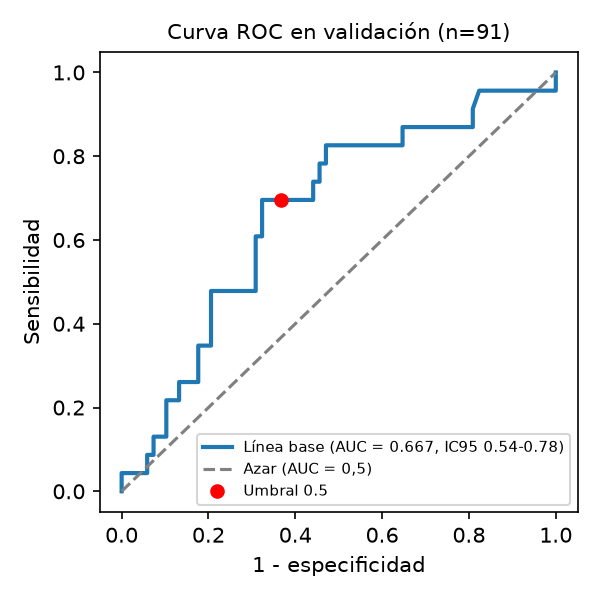
\includegraphics[width=0.48\textwidth]{figuras/curva_roc.png}\hfill
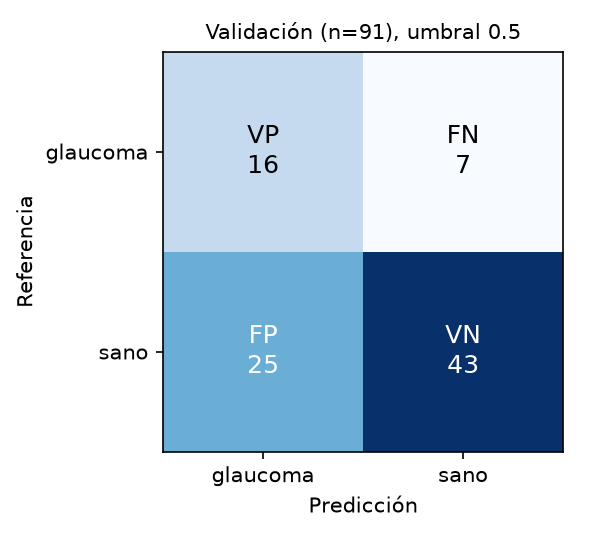
\includegraphics[width=0.48\textwidth]{figuras/matriz_confusion.png}
\caption{Curva ROC en validación, con el punto de operación del umbral 0,5 (izquierda), y matriz de confusión con conteos (derecha)}\label{fig:roc}
\end{figure}

\subsection*{Casos ilustrativos}

La Figura~\ref{fig:casos} muestra tres casos independientes de la validación con su imagen, la etiqueta de referencia, la probabilidad estimada y la predicción. Son solo ilustraciones: las métricas anteriores se calcularon con las 91 imágenes. La tabla con todos los casos (código, referencia, probabilidad y predicción) está en \texttt{predicciones\_validacion.csv} y se resume en el Anexo~\ref{secA1}.

\begin{figure}[h]
\centering
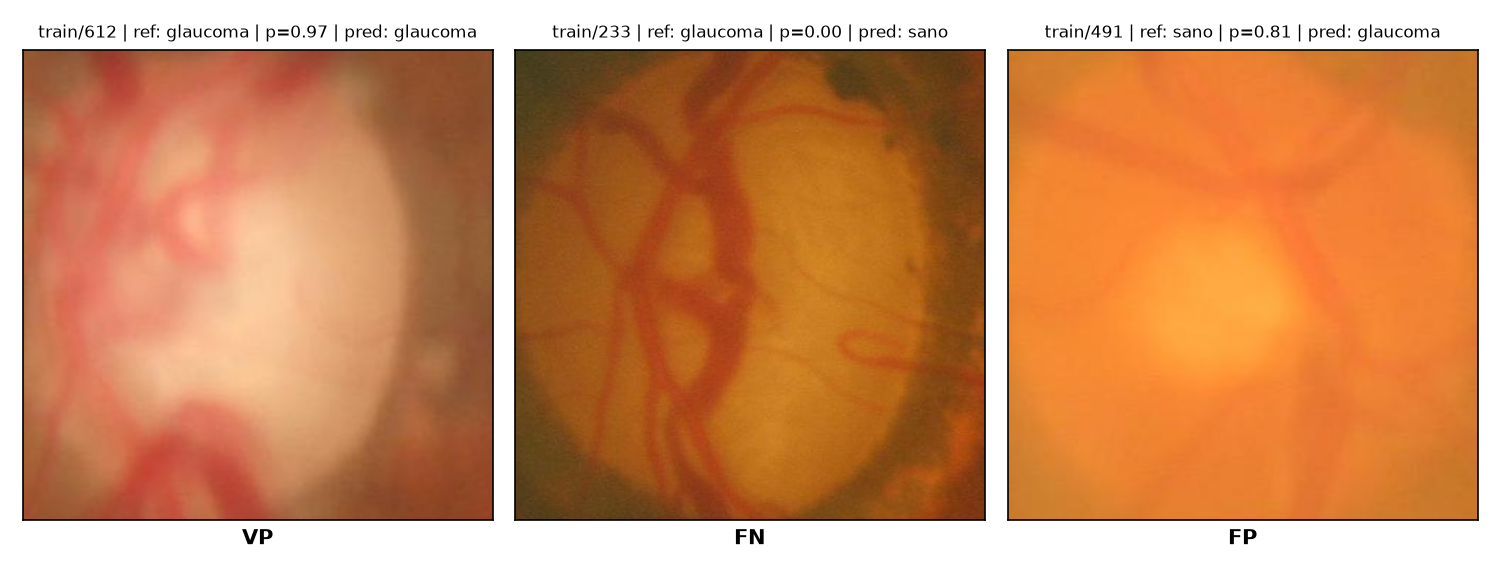
\includegraphics[width=\textwidth]{figuras/casos_validacion.png}
\caption{Tres casos de validación: un verdadero positivo (\texttt{train/612}), un falso negativo (\texttt{train/233}) y un falso positivo (\texttt{train/491}). En cada tipo se tomó el caso con la probabilidad más extrema. Sobre cada imagen: código, etiqueta de referencia, probabilidad de glaucoma estimada y predicción con umbral 0,5}\label{fig:casos}
\end{figure}

\subsection*{Análisis de un error}

Elegimos un falso negativo, porque es el error de mayor costo en tamizaje, y entre ellos el más marcado.

\begin{itemize}
\item \textbf{Dónde difiere:} caso \texttt{train/233}, referencia 1 (glaucoma), probabilidad 0,004, predicción 0 (sano). Los otros 6 FN quedaron cerca del umbral ($p$ entre 0,39 y 0,49); este es el único que el modelo descarta con total seguridad.
\item \textbf{Qué se observa en la imagen:} es una toma más oscura y amarillenta que el resto (Figura~\ref{fig:casos}, centro), con bordes oscuros, el disco ocupando casi todo el recorte y vasos gruesos que lo cruzan. En las características, su \texttt{media\_R} es 0,71, cuando en entrenamiento el mínimo es 0,87 y la media 0,992 (desviación 0,011): queda a 26,6 desviaciones de la media. Su \texttt{media\_G} también es más baja que la de todas las imágenes de entrenamiento.
\item \textbf{Hipótesis:} el error lo causa la exposición de la toma y no el disco. Como el canal rojo casi siempre está saturado, \texttt{media\_R} apenas varía en entrenamiento; una imagen oscura con el rojo sin saturar produce un valor estandarizado extremo, y la regresión, al ser lineal, lo extrapola. Solo el término de \texttt{media\_R} aporta $-$6,6 al logit, y el de \texttt{media\_G}, $-$2,2. Es una hipótesis, no una causa demostrada.
\item \textbf{Prueba para comprobarla:} (1) Sin reentrenar, recortar cada característica de este caso al rango visto en entrenamiento y volver a predecir. Lo hicimos (\texttt{06\_analisis\_error.py}, salida en \texttt{analisis\_error.txt}): la probabilidad sube de 0,004 a 0,18. La extrapolación explica que el error sea tan seguro, pero no el error en sí, porque el caso sigue clasificado como sano. (2) Para la parte restante, la prueba es normalizar el brillo de cada imagen antes de medir (por ejemplo, dividir cada canal por su media en el disco) o quitar \texttt{media\_R}, reentrenar \emph{solo} con entrenamiento y comprobar con validación cruzada dentro de entrenamiento si el AUC se mantiene, y si \texttt{train/233} supera el umbral. Si lo supera, la causa es la exposición; si no, el caso necesita una representación de la forma de la copa que estas medidas no capturan.
\end{itemize}

%%==================================================================%%
\section{Próximo paso}\label{sec:siguiente}
%%==================================================================%%

\textbf{Cambio principal.} Reemplazar las 8 características hechas a mano por características aprendidas. Usaremos una red convolucional preentrenada en ImageNet, ResNet-18 \cite{he2016resnet}, como extractor fijo y mantendremos el mismo clasificador (regresión logística balanceada). Así el único cambio es la representación de la imagen, y la comparación con la línea base es directa. La hipótesis es que la red capta detalles que nuestras medidas de brillo no ven, como la forma del borde de la copa o el recorrido de los vasos sobre el disco.

\textbf{Contra qué se compara.} Contra la línea base de este informe, con la misma partición, la misma semilla y las mismas 91 imágenes de validación. Solo el modelo que se elija al final se evaluará una vez sobre la prueba reservada, sin las 4 imágenes que tienen un gemelo en entrenamiento (192 imágenes; Sección~\ref{sec:particion}).

\textbf{Métrica de mejora.} El AUC-ROC en validación como criterio principal. Como criterio secundario, la sensibilidad con el umbral ajustado para no bajar de la especificidad obtenida por la línea base.

\textbf{Error a vigilar.} Los falsos negativos, y en particular si el caso analizado en la Sección~\ref{sec:piloto} (\texttt{train/233}) se corrige o se mantiene. Como la línea base respondió sobre todo al brillo general, revisaremos también si la red es sensible a la exposición, comparando sus errores en las tomas más oscuras y más claras. Además vigilaremos el sobreajuste, comparando el AUC de entrenamiento con el de validación, porque con 363 imágenes y 512 características por imagen el riesgo de sobreajuste es mucho mayor que con 8.

\begin{table}[h]
\caption{Responsables y aporte verificable de cada integrante}\label{tab:roles}
\begin{tabularx}{\textwidth}{@{}L{3.4cm}XX@{}}
\toprule
Integrante & Aporte en esta entrega & Responsabilidad para la entrega final \\
\midrule
Giuseppe Kanyike Buwule & \pendiente{p.\,ej., script de inventario y partición} & \pend \\
Daniel Duque & \pendiente{p.\,ej., línea base y métricas} & \pend \\
Juan David Daza & \pendiente{p.\,ej., estado del arte e informe} & \pend \\
\botrule
\end{tabularx}
\footnotetext{Cada aporte se puede verificar en los archivos del ZIP de evidencias indicados en el Anexo~\ref{secA2}.}
\end{table}

\backmatter

\bibliography{referencias}

\begin{appendices}

\section{Resultados por caso en validación}\label{secA1}

La Tabla~\ref{tab:errores} lista los 32 errores de validación con su probabilidad estimada. Los 59 aciertos (16 VP y 43 VN) y las columnas completas (código, referencia, probabilidad, predicción y tipo) están en \texttt{predicciones\_validacion.csv}. Todos los códigos son de la carpeta \texttt{ORIGA/train}.

\begin{table}[h]
\caption{Errores en validación con umbral 0,5: código de imagen y, entre paréntesis, la probabilidad de glaucoma estimada, ordenados de menor a mayor}\label{tab:errores}
\begin{tabularx}{\textwidth}{@{}L{2.4cm}X@{}}
\toprule
Tipo & Casos \\
\midrule
FN (7): glaucoma predicho como sano & 233 (0,00), 208 (0,40), 617 (0,40), 336 (0,43), 605 (0,46), 646 (0,48), 589 (0,48) \\
\midrule
FP (25): sano predicho como glaucoma & 649 (0,50), 082 (0,50), 493 (0,51), 064 (0,51), 350 (0,52), 303 (0,52), 288 (0,53), 481 (0,53), 633 (0,53), 259 (0,53), 032 (0,54), 073 (0,55), 371 (0,55), 547 (0,57), 192 (0,57), 217 (0,58), 075 (0,59), 146 (0,60), 282 (0,62), 287 (0,62), 167 (0,64), 606 (0,65), 177 (0,68), 509 (0,68), 491 (0,81) \\
\botrule
\end{tabularx}
\end{table}

\section{Contenido del ZIP de evidencias y cómo ejecutarlo}\label{secA2}

El archivo \texttt{E2\_Proyecto\_B\_Equipo\pendiente{XX}\_2026-30\_Evidencias.zip} contiene:

{\raggedright
\begin{itemize}
\item \texttt{README.md}: instrucciones de instalación y ejecución.
\item \texttt{requirements.txt} y \texttt{config.yaml}: dependencias, semilla, parámetros y la conclusión de la revisión visual de los pares sospechosos.
\item \texttt{comun.py} (lectura de la configuración), \texttt{01\_inventario.py}, \texttt{02\_particion.py}, \texttt{03\_verificar\_particion.py}, \texttt{04\_linea\_base.py}, \texttt{05\_figuras.py}, \texttt{06\_analisis\_error.py}.
\item \texttt{resultados/}: \texttt{inventario.csv}, \texttt{particion.csv}, \texttt{verificacion\_particion.txt}, \texttt{revision\_pares.csv}, \texttt{prueba\_excluidos.csv}, \texttt{caracteristicas.csv}, \texttt{predicciones\_validacion.csv}, \texttt{metricas\_validacion.json}, \texttt{analisis\_error.txt}.
\item \texttt{figuras/}: \texttt{casos\_validacion.png}, \texttt{matriz\_confusion.png}, \texttt{curva\_roc.png}, \texttt{caracteristicas\_por\_clase.png}, \texttt{pares\_phash.png}, \texttt{pares\_consecutivos.png} y \texttt{pares\_mismo\_ojo.png}.
\end{itemize}
}

El conjunto de datos no se incluye (ver Sección~\ref{sec:datos}). Para ejecutar el trabajo se descarga la copia de Kaggle, se ubica la carpeta \texttt{archive/} en la ruta indicada en \texttt{config.yaml} y se corren los scripts del 01 al 06 en orden, como explica \texttt{README.md}. Todo el proceso tarda menos de un minuto en CPU.

\end{appendices}

\end{document}
